\pdfminorversion=6 % this is needed to be able to include pdf 1.6. 
                    % For some reasons some old HPSG proceedings have pdf 1.6
\documentclass[a4paper,11pt]{article}
\usepackage{times}
\usepackage{ogonek} % Dąbkowski
\hyphenation{Acad-e-my}
\usepackage{pdfpages}
\pdfinclusioncopyfonts=1
\usepackage[utf8]{inputenc}
        \usepackage{hyperref}
        \hypersetup{colorlinks=false, pdfborder={0 0 0}}
        \setcounter{page}{274}
        \begin{document}

\newcommand\formatauthor[2]{\begin{tabular}[t]{@{}c@{}}
  {\LARGE#1\strut}\\
  {\small#2\strut}\\
  \rule{\dimexpr0.5\linewidth-1em}{0pt}
  \end{tabular}\xhfill\ignorespaces}
\newcommand\xhfill{\hspace{1em plus 1fill}}
\thispagestyle{empty}

\begin{center}
  {\huge\bfseries A Trace Analysis of Korean UDCs\par}

  \bigskip

~\\
\begingroup
\setlength{\leftskip}{0pt plus 1fill}
\setlength{\rightskip}{0pt plus 1fill}
\setlength{\parindent}{0pt}
\setlength{\parfillskip}{0pt}
  \formatauthor{Sun-Hee Lee}{\begin{tabular}{@{}c@{}}Wellesley College\end{tabular}}

\par\endgroup

  \vspace*{8ex}

  Proceedings of the 12th International Conference on\par Head-Driven Phrase Structure Grammar

  \bigskip

  Department of Informatics, University of Lisbon

  \medskip

  Stefan Müller (Editor)

  \medskip

  2005

  \medskip

  CSLI Publications

  \medskip

  pages 274--289

  \medskip

  \url{http://csli-publications.stanford.edu/HPSG/2005}
\end{center}
\vfill

\noindent
Keywords: 8211; in the traditional HPSG analysis of
UDCs following Pollard and Sag (1994). It is because in HPSG traces 
are not all required to have the same feature, unlike in other
movement-based approaches including the minimalist program and GB
theory. In addition, we argue that the three kinds of Korean UDC
elements appearing in gap positions do not form separate categories
from their corresponding forms appearing in non-UDCs based on the
same semantic and pragmatic properties such as logophoricity and
contrastiveness. We also investigate some controversial issues of
island constraints and strong crossover with respect to filler-gap
linkage in Korean UDCs.


\vfill
\noindent
% APA Style
Lee, Sun-Hee. 2005. A Trace Analysis of Korean UDCs. In Müller, Stefan (Ed.), \emph{{Proceedings of the 12th International Conference on Head-Driven Phrase Structure Grammar, Department of Informatics, University of Lisbon}}, 274--289. Stanford,
CA: CSLI Publications. \hfill\href{http://creativecommons.org/licenses/by/4.0/}{\includegraphics[height=.75em]{Includes/ccby.eps}}

\newpage
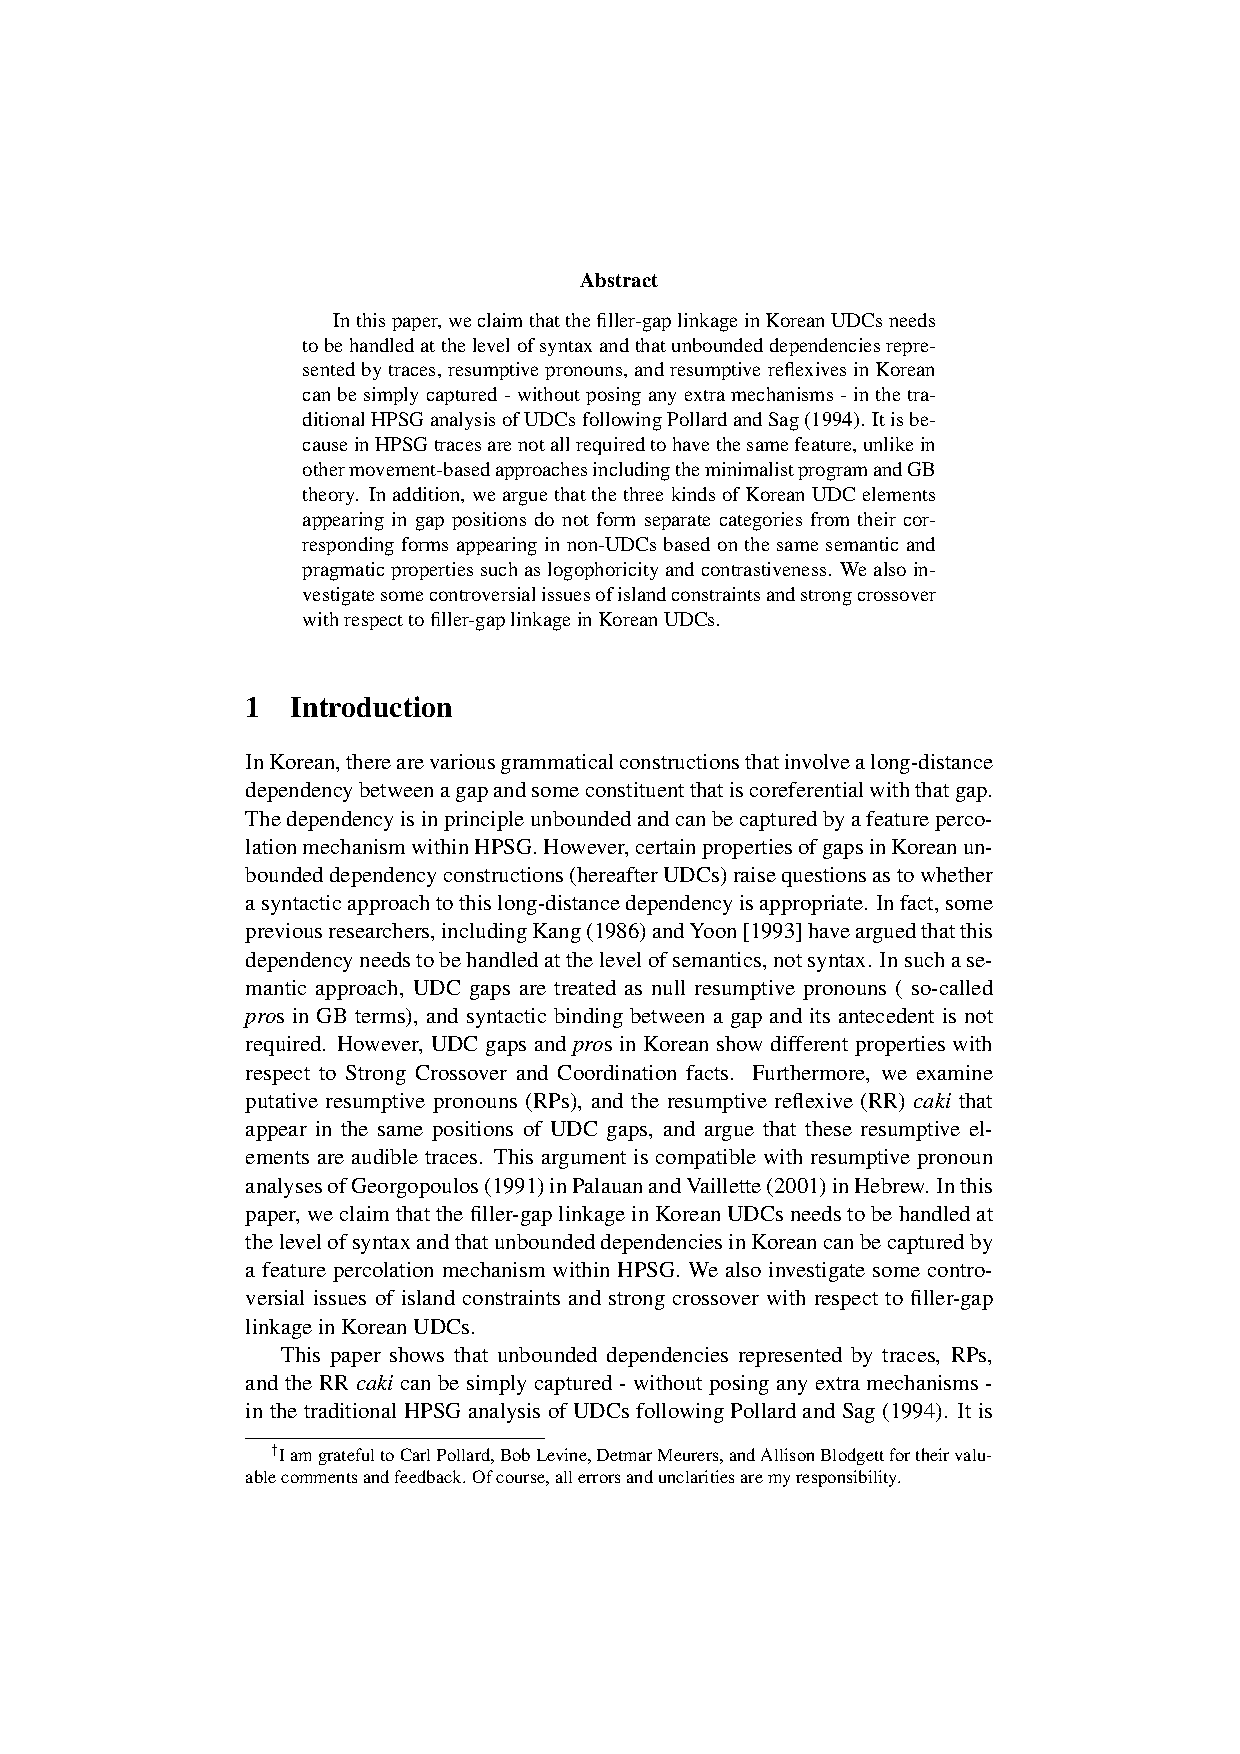
\includepdf[pages=-,pagecommand=\thispagestyle{plain}]{Includes/lee.pdf}
        \end{document}
